\documentclass{article}
\usepackage{graphicx} % Required for inserting images
\usepackage{tikz}
\usepackage{float}
\usepackage{url}
\usepackage{amsmath}
\usepackage{hyperref}
\usepackage{pgfplots}
\usetikzlibrary{positioning}
\pgfplotsset{compat=1.18}


\begin{document}

\begin{titlepage}
    \centering

    \noindent
    \begin{minipage}[t]{0.55\textwidth}
        \raggedright
        \includegraphics[height=1.6cm]{SG.png}\hspace{0.5em}%
    \end{minipage}%
    \hfill
    \begin{minipage}[t]{0.35\textwidth}
        \raggedleft
        \includegraphics[height=1.6cm]{mines.png}
    \end{minipage}

    \vspace{1cm}

    \noindent
    {\color{violetstage}\bfseries\large Benguedda --Lauzon Elias}\\[0.2em]

    \vspace{0.8cm}

    \noindent
    {\color{violetstage}\bfseries\scshape École nationale supérieure des mines de Saint-Étienne}\\[0.2em]
    {\color{violetstage}\bfseries 158 Cours Fauriel, 42023 Saint-Étienne cedex 2}

    \vspace{3cm}

    {\color{violetstage}\bfseries\Large Rapport de stage « Assistant-ingénieur »}\\[1em]
    {\color{violetstage}\bfseries\large Recherche Quantitative}\\[1.5em]
    {\color{violetstage}\bfseries\large Callable Bonds}\\[1.5em]


    \vfill

    \begin{flushleft}
    {\color{violetstage}\bfseries Entreprise d'accueil :} Société Générale, Pricing Team, \\
    Adresse(s) : 15 Parvis de la Défense, 92800 Puteaux.\\[0.6em]
    {\color{violetstage}\bfseries Tuteur Entreprise :} KONE Lanzeni (Ingénieur Pricing)\\[0.6em]
    {\color{violetstage}\bfseries Enseignant référent :} RULLIERE Didier
    \end{flushleft}

\end{titlepage}



\tableofcontents



\clearpage

\section*{Acknowledgements}

I would like to express my sincere gratitude to all the people who contributed to making this experience both enriching and rewarding.

First, I would like to thank my supervisor, Kone L., for their guidance, availability, and valuable advice throughout this experience. Their support and feedback allowed me to progressively develop my skills and gain a better understanding of the professional environment.

I would also like to thank the members of the Pricing Team for their warm welcome, their support, and the time they dedicated to answering my questions and sharing their knowledge. Working alongside them was an important part of this experience and allowed me to discover new professional and technical perspectives.


Finally, I would like to thank everyone who, directly or indirectly, contributed to this experience and helped make it a valuable step in my academic and professional development.
\clearpage

\section{Description of the company}

Société Générale (SG) is one of the four major banking groups in France. It was founded in 1864 and is a banking group whose activities are divided into two groups retail banking and investment banking. The group is present internationally through offices all around the world and employs more than 100,000 people worldwide. Its turnover is around \$ 25 Billion per year. 

Société Générale Securities Servicies (SGSS) is a subsidiary of the Société Générale Group specialized in securities services and providing solutions to financial institutions. Its activities are part of what we call in bank middle and front office activities.

My internship took place within SGSS in the Pricing Team desk. The team provides pricing services to various financial institutions, including BBVA, Goldman Sachs, J.P. Morgan, and CNP. This pricing activity is a part of the regulatory requirement imposed by the french regulator: the AMF (Autorité des Marchés Financiers) which aims to provide clarity and to ensure transparency of financial products to avoid financial crisis.

The team in which I worked is called Pricing Team. Its main role is therefore to value structured products and OTC derivatives with a quantitative approach. This activity lies at the intersection of quantitative tools and client relationship.



\section{Definition of the objectives}

During my internship, I had the opportunity to work on two projects involving two very different types of financial assets. The first project focused on interest rate securities, and the second one was about equity assets. This report is dedicated to the first project: the pricing of callable bonds. The second project, on correlation modelling, is presented in a separate report.

\subsection{Callable Bonds:}


The objective of this first project was therefore to understand and implement the different components required to price a callable bond, from the valuation of the underlying vanilla bond to the modelling of interest rates and the optimal exercise decision. In particular, I studied the Hull–White one-factor interest rate model (HW1F) and the optimal stopping problem associated with the issuer’s call decision. Depending on the exercise features of the bond, different pricing approaches were considered from analytical methods for European-style exercise to numerical methods based on Monte Carlo simulation.

The developed approaches were implemented using Numerix, the pricing software used by the team.
\\

\subsubsection{Bonds:}


A bond is a fixed-income financial security \footnote{Financial product that mainly depends of interest rates} through which an issuer borrows money from an investor for a predetermined period of time. In exchange the investor receives a series of cash flows according to the terms specified before the emission in the contract. 

A classic bond, also referred to as a vanilla bond, generally consists of two types of cash flows. First, the issuer periodically pays coupon payments to the bondholder. These payments represent the interest paid on the borrowed amount and can be fixed at the beginning of the contract or, depending on the structure of the bond, variable. Second, at the maturity date, the issuer repays the principal, corresponding to the initial amount borrowed.

Here is a simple vizualization for this financial product:


\begin{figure}[H]
    \centering
    \begin{tikzpicture}[>=stealth]

        % Timeline
        \draw[->] (0,0) -- (12,0) node[right] {Time};
        
        % Initial investment
        \draw (10,0.1) -- (10,-0.1);
        \draw[->] (0,0.1) -- (0,1.2);
        \node[above] at (0,1.2) {$-N$};
        \node[below] at (0,-0.1) {$t=0$};

        % Coupon dates
        \foreach \x/\i in {
            2/1,
            4/2,
            6/3,
            8/{n-1}
        }{
            \draw (\x,0.1) -- (\x,-0.1);
            \draw[->] (\x,0.1) -- (\x,1.2);
            \node[above] at (\x,1.2) {$C_{\i}$};
            \node[below] at (\x,-0.1) {$T_{\i}$};
        }

        % Maturity
        \draw (10,0.1) -- (10,-0.1);
        \draw[->] (10,0.1) -- (10,1.2);
        \node[above] at (10,1.2) {$C_n+N$};
        \node[below] at (10,-0.1) {$T_n=T$};

    \end{tikzpicture}
    \caption{Cash flows of a vanilla bond}
    \label{fig:bond_cashflows}
\end{figure}



The formula for a bond can be represented as a series of future cash flows occurring at predetermined dates. If the payment dates are denoted by $(T_1, T_2, \ldots, T_n)$, and the corresponding cash flows by $(c_1, c_2, \ldots, c_n)$, the value of the bond at a given time $t$ can be expressed as the present value (discounted value \footnote{Discounted means that a future cash flow is converted into its equivalent value at an earlier date by applying an appropriate discount factor, usually an exponential comounding.}) of these future cash flows:

\begin{equation}
P_{\text{bond}}(t)=\sum_{i=1}^{n} c_i P(t,T_i),
\end{equation}

where $P(t,T_i)$ represents the price at time $t$ of a zero-coupon bond paying one unit of currency at date $T_i$.

\\

This representation is particularly useful for the pricing of callable bonds. Indeed, a callable bond can be viewed as a conventional bond combined with an embedded option that gives the issuer the right to redeem the bond before its maturity. The presence of this option makes the valuation of a callable bond more complex than that of a standard vanilla bond as we will see later.
\\

\subsubsection{Interest rates:}

Interest rates are fundamental in finance. They determine the cost of borrowing/lending. In the context of fixed-income products, interest rates are really important because they are used to determine the present value of future cash flows (as said before for the bond pricing). The value of a financial product therefore depends on the amount, timing of its future cash flows and on the interest rates used to discount them.


Several characteristics are really relevant when we want to find the appropriate interest rate for a financial product. The first one is the maturity, which represents the period of time between the valuation date and the date at which the final cash flow is paid (T). Interest rates always vary depending on the maturity of the product. This relationship between interest rates and maturities is represented by the yield curve \footnote{Example of a yield curve can be find at: \url{https://www.ustreasuryyieldcurve.com}}, which is a fundamental tool for the valuation of fixed-income securities.

In modern financial markets, several reference rates are used to build interest-rate curves. For example, we have: the Overnight Index Swap (OIS) which plays an important role in the valuation of interest-rate derivatives. In the euro area, the main overnight reference rate is the -Euro Short-Term Rate (€STR), while in the United States the ecured Overnight Financing Rate (SOFR) is maily used. LIBOR, which was historically one of the main reference rates used in financial markets, has now been discontinued for the major currencies and replaced by alternative risk-free or nearly risk-free reference rates. But there are a lot of financial products we were working on which were still using this interest rate because they were emitted before 2024.


This relationship between interest rates and bond prices is particularly important for callable bonds. In fact, the value of the embedded call option \footnote{ In this context a call option gives its holder the right, but not the obligation, to (re)buy an asset at a predetermined price before or at a specified date.} depends on the evolution of interest rates and on the possibility for the issuer to refinance its debt under more interesting conditions. Understanding the behavior of interest rates is therefore essential for the valuation of a callable bond.
\\

\subsubsection{Zero-coupon bonds:}

A zero-coupon bond (ZCB) is a fixed-income instrument that pays a single cash flow at maturity T and does not pay any intermediate coupon payments. The holder of the ZCB receives only one payment at the maturity date. Zero-coupon bond is a fundamental building block in fixed-income pricing, it permits to represent the value of a future cash flow.

The price of a zero-coupon bond is mainly determined by the interest rate corresponding to its maturity. If $P(t,T)$ denotes the price at time $t$ of a zero-coupon bond paying one unit of currency at maturity $T$, its value can be interpreted as the present value of this future payment. In a simplified setting with a constant continuously compounded interest rate $r$, the price can be written as:
\begin{equation}
    P(t,T) = e^{-r(T-t)}.
\end{equation}
In practice, interest rates are not constant and depend on the maturity. The prices of zero-coupon bonds can therefore be used to construct the discount curve, which represents the value today of receiving one unit of currency at different future dates.

Zero-coupon bonds are particularly important in the valuation of fixed-income derivatives because future cash flows can be discounted using the corresponding zero-coupon bond prices. For example, the price of a vanilla bond can be expressed as the sum of the present values of all its future coupon payments and its principal repayment:
\begin{equation}
    B(t) = \sum_{i=1}^{n} C_i P(t,T_i) + N P(t,T_n),
\end{equation}
where $C_i$ represents the coupon paid at date $T_i$ and $N$ is the nominal value of the bond.

Zero-coupon bonds also play a central role in the valuation of callable bonds. Indeed, the underlying bond can be decomposed into a set of future cash flows, each of which can be discounted using the appropriate zero-coupon bond price. Moreover, in interest-rate models such as the Hull--White model, zero-coupon bond prices are used to describe the evolution of interest rates and to derive the value of interest-rate derivatives. They therefore provide an essential link between the observed market yield curve and the theoretical pricing framework used for callable bonds.
\\


\subsubsection{Callable Bonds}

The financial product that I studied during my internship is a callable bond. A callable bond has the same structure as the vanilla bond but with more callability dates.

The dates on which the issuer is allowed to exercise this right, as well as the corresponding redemption price, are specified in the Term Sheet \cite{SGTermSheet} of the product. In the framework of this project, we assumed that the bond could be called at par, meaning that the issuer repays the notional amount of the bond without any additional premium.
Moreover, we will use only endogenous phenomena because it is a lot more difficult to quantify the cash needs of the issuer. For example a lender could want to recall the callable bond for its report but these kind of phenomena are exogenous.
Depending on the number and frequency of the possible exercise dates, callable bonds can be into three main categories.

\begin{itemize}
    \item \textbf{European callable bond:} the issuer has only one possible call date during the life of the bond. The call option can therefore only be exercised at a single predetermined date.

    \item \textbf{Bermudan callable bond:} the issuer can exercise the call option on a finite number of predetermined dates. For example, the bond may be callable every three months or on a specific date at the beginning of each year during a given period.

    \item \textbf{American callable bond:} the issuer can exercise the call option at any time during a predefined period. In this case, the set of possible exercise dates is continuous.
\end{itemize}

The distinction between these three types of callable bonds is particularly important. The more frequently the issuer is allowed to exercise the call option, the greater the flexibility provided by the embedded option and then the call option is more expansive. As a result, the valuation of a Bermudan or American callable bond generally requires more advanced numerical methods than the valuation of a European callable bond as we will see later.

\paragraph{Decomposition of a Callable Bond}

A useful way to understand and value a callable bond is to decompose it into a standard vanilla bond and an embedded call option. Consider first a vanilla bond with the same coupon schedule, notional amount, and maturity as the callable bond. Its value at time $t$ is given by the present value of all its future cash flows:

\begin{equation}
P_{\text{bond}}(t)
=
\sum_{i=1}^{n} c_i P(t,T_i),
\end{equation}

where $T_i$ denotes the payment dates, $c_i$ the corresponding cash flows, and $P(t,T_i)$ the price at time $t$ of a zero-coupon bond maturing at $T_i$.
\\

The callable feature can then be interpreted as an option given to the issuer of the bond. Since the issuer owns the right to redeem the bond before maturity, the investor is effectively short \footnote{Being short of an asset means one that one sell the asset without being the owner of it. The opposite is to be long} this embedded call option. Therefore, from the investor's point of view, the value of a callable bond can be expressed as

\begin{equation}
P_{\text{callable}}(t)
=
P_{\text{vanilla}}(t)
-
V_{\text{call}}(t)
\end{equation}

where $V_{\text{call}}(t)$ represents the value of the call option embedded in the bond. The subject of this internship is mainly to calculate the value of this option.
\\

For a European callable bond with a single call date $T_c$, the value of the embedded call option can be expressed using the value of the underlying bond at the exercise date. If $K$ denotes the call price, the payoff of the call option from the issuer's perspective at $T_c$ is

\begin{equation}
\text{Payoff}_{\text{call}}(T_c)
=
\left(
P_{\text{vanilla}}(T_c) - K
\right)^+
=
\max\left(
P_{\text{vanilla}}(T_c) - K,
0
\right)
\end{equation}

The option is therefore valuable when the market value of the underlying bond exceeds the call price. In this situation, the issuer can exercise the call option and redeem the bond at $K$, instead of leaving the bond outstanding at a higher market value.


\begin{equation}
\text{Payoff}_{\text{call}}(T_c)
=
\left(
\sum_{i=1}^{n} c_i P(T_c,T_i) - K
\right)^+
\end{equation}

In the particular case considered in this project, the callable bond is assumed to be callable at par. If $N$ denotes the notional amount of the bond, the call price is therefore given by

\begin{equation}
K=N
\end{equation}

The pricing problem can consequently be summarized by the following decomposition:

\begin{equation}
P_{\text{callable}}(t)
=
\sum_{i=1}^{n} c_i P(t,T_i)
-
V_{\text{call}}(t)
\end{equation}

This decomposition is the starting point for the pricing methodology developed during the internship. The main challenge is therefore to determine the value of the embedded call option, which depends on the evolution of interest rates and, in the case of a Bermudan or American callable bond, on the optimal exercise strategy of the issuer.



\section{Methodologies Used}

This section presents the pricing methodology used for callable bonds and the different numerical and analytical approaches that are used depending on the exercise feature of the product.

The pricing of a callable bond can naturally be
formulated as an optimal stopping problem. The methodology used to
solve this problem depends on the exercise structure of the call
feature. In particular, three cases will be considered:

\begin{itemize}
    \item European callable bonds, for which there is a single
    exercise date and an analytical solution can be obtained using
    Jamshidian's decomposition;
    
    \item Bermudan callable bonds, for which the issuer can exercise
    the call at a finite number of predetermined dates. In this case,
    Monte Carlo simulation combined with the Longstaff--Schwartz
    algorithm can be used to estimate the continuation value;
    
    \item American callable bonds, for which exercise is theoretically
    possible at any time before maturity. This continuous-time optimal
    stopping problem is approximated numerically by discretizing time
    and applying a Monte Carlo regression methodology.
\end{itemize}

\subsection{Callable Bonds}

\subsubsection{The Hull--White One-Factor Model}

In order to price callable bonds, it is first necessary to specify
a model for the evolution of interest rates. The interest-rate model
chosen by the pricing team is the HW1F.

The Hull--White model permits us to modelize the dynamics of the short-term interest rate under the risk-neutral measure $\mathbb{Q}$. The short rate $r_t$ is assumed to follow the stochastic differential equation

\begin{equation}
    dr_t =
    \left(
        \theta(t) - a r_t
    \right)dt
    + \sigma dW_t^{\mathbb{Q}},
\end{equation}

where:

\begin{itemize}
    \item $r_t$ is the instantaneous short-term interest rate at time
    $t$;
    
    \item $a>0$ is the mean-reversion speed of the short rate;
    
    \item $\sigma>0$ is the short-rate volatility;
    
    \item $W_t^{\mathbb{Q}}$ is a standard Brownian motion under the
    risk-neutral measure $\mathbb{Q}$;
    
    \item $\theta(t)$ is a deterministic function chosen to ensure
    that the model is consistent with the initial term structure of
    interest rates.
\end{itemize}

We calibrated all the coefficients of the model using market data. This process is carried out every day thanks to the Numerix system.

The mean-reversion parameter $a$ controls the speed at which the
short rate tends to return towards its time-dependent long-term
level, while $\sigma$ controls the instantaneous volatility of the
short rate.

The function $\theta(t)$ is calibrated such that the model exactly
reproduces the initial zero-coupon bond curve. In terms of the
initial instantaneous forward rate :

\begin{equation}
    f(0,t)
    =
    -\frac{\partial \ln P(0,t)}{\partial t},
\end{equation}

where $P(0,t)$ denotes the market price at time 0 of a zero-coupon bond maturing at time $t$, the drift adjustment is given by : 

\begin{equation}
    \theta(t)
    =
    \frac{\partial f(0,t)}{\partial t}
    +
    a f(0,t)
    +
    \frac{\sigma^2}{2a}
    \left(
        1-e^{-2at}
    \right).
\end{equation}

This calibration property is particularly useful in a pricing
framework since the model is consistent with the market term
structure observed at the valuation date.


% ============================================================
% OPTIMAL STOPPING
% ============================================================

\subsubsection{Callable Bonds as an Optimal Stopping Problem}


The decision of calling the product can be formulated as an optimal stopping problem. Let $V(t,r_t)$ denote the value of the callable bond at time $t$. From the issuer's perspective, the exercise decision consists of comparing the value obtained by calling the bond with the value of continuing to hold the contract.

Let $K(t)$ denote the call price paid by the issuer when the call is
exercised at time $t$. The continuation value can be represented as

\begin{equation}
V^c(t,r_t)
=
\mathbb{E}^{\mathbb{Q}}
\left[
\int_t^{\tau}
e^{-\int_t^s r_u\,du}
C(s)\,ds
+
e^{-\int_t^\tau r_u\,du}
Z(\tau)
\middle|
\mathcal{F}_t
\right],
\end{equation}

where $C(s)$ represents the contractual coupon cash flow and $Z(\tau)$ represents the cash flow received at the stopping time $\tau$.

The payoff at the stopping time can be written as

\begin{equation}
Z(\tau)
=
\begin{cases}
K(\tau), & \text{if } \tau<T,\\
N, & \text{if } \tau=T,
\end{cases}
\end{equation}

where $N$ denotes the nominal value of the bond.

The optimal exercise time is therefore the stopping time at which
the issuer decides to exercise the call rather than continue the
contract. It can be formally represented as

\begin{equation}
\tau^*
=
\inf
\left\{
s\geq t:
V^c(s,r_s)\geq K(s)
\right\}.
\end{equation}

The exact interpretation of the inequality depends on the
perspective and sign convention adopted for the value of the
callable bond. Economically, the issuer exercises when the benefit
of redeeming the bond is greater than the value associated with
continuing the contract.

The pricing methodology then depends on the set of admissible
stopping times. Three different cases are considered below.


% ============================================================
% EUROPEAN
% ============================================================

\subsubsection{European Callable Bonds}

A European callable bond can only be called at a single predefined
date $T_c$. Therefore, there is no exercise-time optimization over
several dates. The problem can consequently be transformed into a
portfolio of European options and solved analytically in the
Hull--White framework. This is the simplest case and provides a useful benchmark for the numerical methods used later for Bermudan and American callable bonds.
\\

Under the Hull--White one-factor model, the price at time $t$ of a
zero-coupon bond maturing at time $T$ admits the following
closed-form representation:

\begin{equation}
    P(t,T)
    =
    A(t,T)
    \exp\left(
        -B(t,T)r_t
    \right),
\end{equation}

where

\begin{equation}
    B(t,T)
    =
    \frac{1-e^{-a(T-t)}}{a},
\end{equation}

and

\begin{equation}
    A(t,T)
    =
    \frac{P(0,T)}{P(0,t)}
    \exp
    \left[
        B(t,T)f(0,t)
        -
        \frac{\sigma^2}{4a}
        B(t,T)^2
        \left(
            1-e^{-2at}
        \right)
    \right].
\end{equation}

This affine representation is one of the main advantages of the
Hull--White model. In particular, it allows the price of interest
rate derivatives to be expressed in terms of zero-coupon bond
prices.


\paragraph{Jamshidian's Decomposition.}

For a European callable bond, the call feature can be decomposed
into a portfolio of options on zero-coupon bonds using
Jamshidian's trick \cite{Jashmidian}.

Consider a bond with contractual cash flows $c_i$ paid at dates
$T_1,\ldots,T_n$, with

\begin{equation}
    T_c \leq T_1 < \cdots < T_n.
\end{equation}

At the call date $T_c$, the value of the underlying bond is

\begin{equation}
    V(T_c,r_{T_c})
    =
    \sum_{i=1}^{n}
    c_i P(T_c,T_i;r_{T_c}).
\end{equation}

Using the affine representation of the zero-coupon bond price,

\begin{equation}
    V(T_c,r)
    =
    \sum_{i=1}^{n}
    c_i
    A(T_c,T_i)
    \exp
    \left(
        -B(T_c,T_i)r
    \right).
\end{equation}

The critical short rate $r^*$ is defined as the unique solution of

\begin{equation}
    \sum_{i=1}^{n}
    c_i
    A(T_c,T_i)
    \exp
    \left(
        -B(T_c,T_i)r^*
    \right)
    =
    K.
\end{equation}

For each cash flow $c_i$, we then define

\begin{equation}
    K_i
    =
    P(T_c,T_i;r^*)
    =
    A(T_c,T_i)
    \exp
    \left(
        -B(T_c,T_i)r^*
    \right).
\end{equation}

Consequently, the callable bond can be decomposed into a portfolio
of options on zero-coupon bonds.


\paragraph{European Option on a Zero-Coupon Bond.}

The price at time $t\leq T_c$ of a European call option with expiry
date $T_c$, underlying zero-coupon bond maturity $T_i$ and strike
$K_i$ is given by

\begin{equation}
    \mathrm{ZBC}(t,T_c,T_i,K_i)
    =
    P(t,T_i)N(d_{1,i})
    -
    K_iP(t,T_c)N(d_{2,i}),
\end{equation}

where $N(\cdot)$ denotes the cumulative distribution function of a
standard normal random variable, and

\begin{align}
    d_{1,i}
    &=
    \frac{
        \ln
        \left(
            \frac{P(t,T_i)}
            {K_iP(t,T_c)}
        \right)
    }{\sigma_{P,i}}
    +
    \frac{1}{2}\sigma_{P,i},
    \\[6pt]
    d_{2,i}
    &=
    d_{1,i}-\sigma_{P,i}.
\end{align}

The integrated volatility is

\begin{equation}
    \sigma_{P,i}
    =
    \sigma
    B(T_c,T_i)
    \sqrt{
        \frac{
            1-e^{-2a(T_c-t)}
        }{2a}
    }.
\end{equation}

The value of the European callable bond can therefore be obtained
by subtracting the value of the call option from the value of the
corresponding non-callable bond:

\begin{equation}
    V_{\mathrm{callable}}(t)
    =
    \sum_{i=1}^{n}
    c_iP(t,T_i)
    -
    \sum_{i=1}^{n}
    c_i
    \mathrm{ZBC}(t,T_c,T_i,K_i).
\end{equation}

Equivalently,

\begin{equation}
\begin{aligned}
    V_{\mathrm{callable}}(t)
    =
    \sum_{i=1}^{n}c_iP(t,T_i)
    -
    \sum_{i=1}^{n}c_i
    \Big[
        P(t,T_i)N(d_{1,i})
        -
        K_iP(t,T_c)N(d_{2,i})
    \Big].
\end{aligned}
\end{equation}

This analytical result provides an exact benchmark for the
European case and will be usefull for comparision with the Monte Carlo method as we will see later. European callable bonds represent more than 80\% of the callable bond the pricing team prices everyday.


% ============================================================
% BERMUDAN
% ============================================================

\subsubsection{Bermudan Callable Bonds}

The Bermudan case is more complex than the European case because
the issuer can exercise the call at several predetermined dates.

Let the set of admissible call dates be

\begin{equation}
    \mathcal{T}_c
    =
    \left\{
        T_{c,1},
        T_{c,2},
        \ldots,
        T_{c,m}
    \right\},
\end{equation}

with

\begin{equation}
    t
    \leq
    T_{c,1}
    <
    T_{c,2}
    <
    \cdots
    <
    T_{c,m}
    \leq T.
\end{equation}

At each call date $T_{c,j}$, the issuer has to compare the value
obtained by exercising immediately with the value obtained by
continuing the contract.

The exercise decision can therefore be expressed as

\begin{equation}
    V(T_{c,j},r_{T_{c,j}})
    =
    \min
    \left(
        K(T_{c,j}),
        V^c(T_{c,j},r_{T_{c,j}})
    \right),
\end{equation}

under the issuer's perspective and the convention adopted above.

The continuation value is defined as

\begin{equation}
    V^c(T_{c,j},r_{T_{c,j}})
    =
    \mathbb{E}^{\mathbb{Q}}
    \left[
        D(T_{c,j},T_{c,j+1})
        V(T_{c,j+1},r_{T_{c,j+1}})
        \middle|
        \mathcal{F}_{T_{c,j}}
    \right],
\end{equation}

where the stochastic discount factor is

\begin{equation}
    D(t,T)
    =
    \exp
    \left(
        -\int_t^T r_s\,ds
    \right).
\end{equation}

Unlike the European case, the continuation value is generally not
available in closed form because of the non lineraity of the function $\longmapsto max(.)$. A numerical approximation is therefore
required.


The first step consists in simulating a large number $M$ of paths
of the short rate under the risk-neutral measure, using the HW1F model calibrated with market data.

For each simulated path $m$, the Hull--White dynamics can be
discretized as

\begin{equation}
    r_{t+\Delta t}
    =
    r_t
    +
    \left(
        \theta(t)-ar_t
    \right)\Delta t
    +
    \sigma\sqrt{\Delta t}Z,
\end{equation}

where Z is normally distributed. The integral of the short rate is also approximated along each path in order to compute the corresponding discount factors.

A direct Monte Carlo estimate of the continuation value would
require conditioning on the current short rate. This conditional
expectation is not directly observable from the simulated paths.

% ============================================================
% AMERICAN
% ============================================================

\subsubsection{American Callable Bonds}

The American callable bond represents the most general exercise
feature considered in this study. Contrary to the Bermudan case,
where exercise is restricted to a finite set of dates, the issuer
can theoretically exercise the call at any time before maturity. However, we assume that the product can be called only once a day.

The set of admissible stopping times is therefore
\begin{equation}
\tau \in[t,T].
\end{equation}

The pricing problem becomes a continuous-time optimal stopping
problem. The issuer must determine the optimal stopping time
$\tau^*$ such that exercising the call maximizes the economic
benefit associated with terminating the contract.

In this case, an analytical solution is generally not available once again due to the non linearity of the max function.

A numerical approximation is therefore required.

\paragraph{Time Discretization.}

In practice, the continuous exercise interval is discretized into a
finite time grid:

\begin{equation}
    t=t_0
    <
    t_1
    <
    \cdots
    <
    t_M=T.
\end{equation}

The American exercise problem can then be approximated by a
Bermudan problem in which the issuer is allowed to exercise at each
point of the time grid.

\begin{equation}
    \Delta t
    =
    1\ day
\end{equation}


The same Monte Carlo framework as for the Bermudan callable bond
can therefore be applied.

First, a large number of short-rate paths are simulated under the
risk-neutral measure. For each path, the corresponding discount
factors and bond cash flows are calculated.

At each exercise time $t_j$, the continuation value is estimated
using a regression:

\begin{equation}
    \widehat{V}^c(t_j,r)
    =
    \sum_{k=0}^{K}
    \beta_{j,k}\phi_k(r).
\end{equation}

The issuer then compares the immediate exercise value with the
estimated continuation value. The optimal exercise strategy is
obtained through backward induction.

The backward induction method consists in determining the optimal
exercise decision starting from the last possible call date and
working backwards towards the valuation date. At the final call date,
there is no future call decision to consider, so the value of the
callable bond can be determined directly by comparing the redemption
price with the value of keeping the bond outstanding. This information
is then used to calculate the continuation value at the previous call
date. At each exercise date $t_i$, the issuer compares the immediate
redemption value $K_i$ with the continuation value $C(t_i)$, which
represents the value of not exercising the call and keeping the bond
outstanding. From the investor's point of view, the value of the
callable bond at a call date can therefore be written as

\begin{equation}
V_{\text{callable}}(t_i)
=
\min\left(K_i, C(t_i)\right).
\end{equation}

If the redemption price is lower than the continuation value, the
issuer has an economic incentive to exercise the call and redeem the
bond. Conversely, if the continuation value is lower than the
redemption price, it is preferable for the issuer not to exercise the
call. The value obtained at each exercise date is then used to
calculate the continuation value at the previous date. This process
is repeated backwards until the initial valuation date is reached.
This iterative procedure is referred to as \textit{backward
induction}.

\begin{figure}[H]
\centering

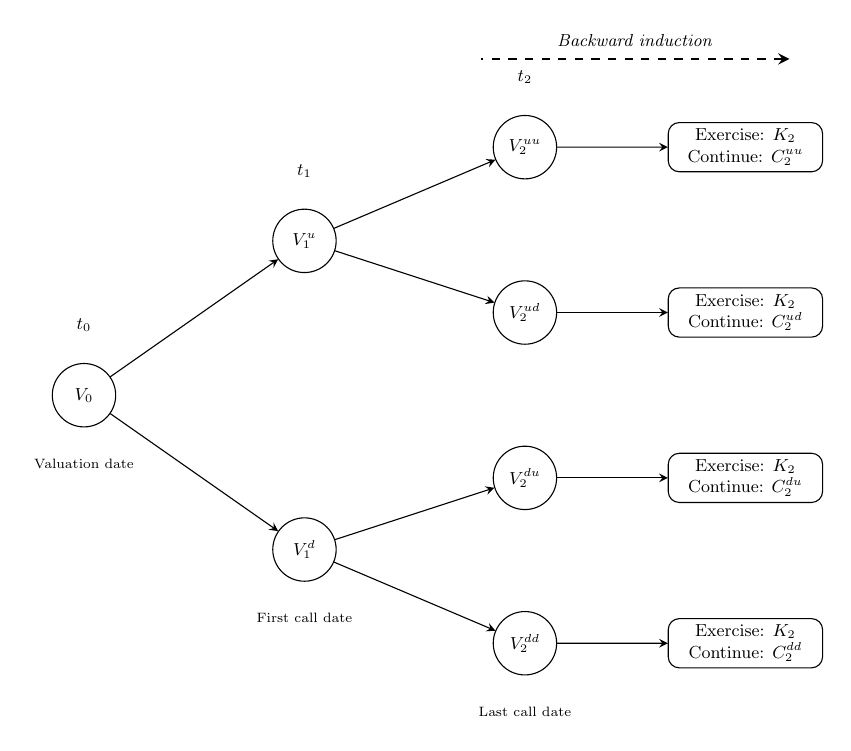
\begin{tikzpicture}[
    scale=0.7,
    transform shape,
    >=stealth,
    every node/.style={font=\small},
    state/.style={
        circle,
        draw,
        minimum size=1.15cm,
        inner sep=2pt,
        align=center
    },
    decision/.style={
        rectangle,
        draw,
        rounded corners,
        align=center,
        minimum width=2.8cm,
        minimum height=0.8cm
    }
]

% ============================================================
% NODES
% ============================================================

% Initial valuation date
\node[state] (V0) at (0,0) {$V_0$};

% First call date
\node[state] (V1u) at (4,2.8) {$V_1^u$};
\node[state] (V1d) at (4,-2.8) {$V_1^d$};

% Last call date
\node[state] (V2uu) at (8,4.5) {$V_2^{uu}$};
\node[state] (V2ud) at (8,1.5) {$V_2^{ud}$};
\node[state] (V2du) at (8,-1.5) {$V_2^{du}$};
\node[state] (V2dd) at (8,-4.5) {$V_2^{dd}$};

% ============================================================
% TIME LABELS
% ============================================================

\node[above=0.45cm of V0] {\textbf{$t_0$}};
\node[above=0.45cm of V1u] {\textbf{$t_1$}};
\node[above=0.45cm of V2uu] {\textbf{$t_2$}};

\node[below=0.45cm of V0]
{\scriptsize Valuation date};

\node[below=0.45cm of V1d]
{\scriptsize First call date};

\node[below=0.45cm of V2dd]
{\scriptsize Last call date};

% ============================================================
% TREE
% ============================================================

\draw[->] (V0) -- (V1u);
\draw[->] (V0) -- (V1d);

\draw[->] (V1u) -- (V2uu);
\draw[->] (V1u) -- (V2ud);

\draw[->] (V1d) -- (V2du);
\draw[->] (V1d) -- (V2dd);

% ============================================================
% DECISION BOXES
% ============================================================

\node[decision] (Duu) at (12,4.5)
{
Exercise: $K_2$\\
Continue: $C_2^{uu}$
};

\node[decision] (Dud) at (12,1.5)
{
Exercise: $K_2$\\
Continue: $C_2^{ud}$
};

\node[decision] (Ddu) at (12,-1.5)
{
Exercise: $K_2$\\
Continue: $C_2^{du}$
};

\node[decision] (Ddd) at (12,-4.5)
{
Exercise: $K_2$\\
Continue: $C_2^{dd}$
};

% ============================================================
% DECISION ARROWS
% ============================================================

\draw[->] (V2uu) -- (Duu);
\draw[->] (V2ud) -- (Dud);
\draw[->] (V2du) -- (Ddu);
\draw[->] (V2dd) -- (Ddd);

% ============================================================
% BACKWARD INDUCTION
% ============================================================

\draw[
    <-,
    thick,
    dashed
]
(12.8,6.1) -- (7.2,6.1)
node[midway, above=0.1cm]
{\textit{Backward induction}};

% ============================================================
% FORMULA
% ============================================================

\end{tikzpicture}

\caption{Illustration of the backward induction method for a Bermudan callable bond.}
\label{fig:backward_induction}
\end{figure}

The estimated American callable bond price can consequently be
written as

\begin{equation}
    \widehat{V}_0^{\mathrm{Am}}
    =
    \frac{1}{M}
    \sum_{m=1}^{M}
    \Pi_0^{(m)},
\end{equation}

where $\Pi_0^{(m)}$ represents the discounted cash flows associated
with the optimal exercise strategy on path $m$.



The main difference between Bermudan and American callable bonds is
therefore the set of admissible exercise times.

For a Bermudan callable bond,

\begin{equation}
    \tau
    \in
    \left\{
        T_{c,1},
        \ldots,
        T_{c,m}
    \right\},
\end{equation}

whereas for an American callable bond,

\begin{equation}
    \tau
    \in
    [t,T].
\end{equation}

From a numerical perspective, the American problem is approximated
by increasing the number of exercise dates in the time grid. The
accuracy of the approximation therefore depends on both the number
of simulated paths and the fineness of the time discretization.

This also makes the American callable bond computationally more
demanding than the Bermudan case. In addition to the Monte Carlo
sampling error, the numerical approximation introduces a time
discretization error and a regression error.


% ============================================================
% COMPARISON OF THE METHODS
% ============================================================

\subsubsection{Comparison of the Pricing Methodologies}

The three callable bond structures can be summarized according to
their exercise features and pricing methodologies.

\begin{table}[h!]
\centering
\begin{tabular}{|c|c|c|}
\hline
\textbf{Product} & \textbf{Exercise Dates} & \textbf{Pricing Method} \\
\hline
European Callable Bond
& One date
& Analytical / Monte Carlo \\
\hline
Bermudan Callable Bond
& Finite set of dates
& Monte Carlo \\
\hline
American Callable Bond
& Continuous interval
& Monte Carlo \\
\hline
\end{tabular}
\caption{Pricing methodologies for the different callable bond structures.}
\label{tab:callable_methods}
\end{table}

The European case provides an analytical benchmark against which
the numerical implementation can be validated. Once the Monte Carlo
framework has been validated, it can be extended to Bermudan and
American callable bonds, for which analytical solutions are
generally unavailable.

\subsection{Conclusion:}

The Pricing Team uses a specific software named Numerix \cite{Numerix}. The implementation of the exact analytical formula in Numerix could not be completed during this first stage of the project. This highlighted some of the limitations of the existing pricing environment and motivated further work on the implementation. In the second period of my internship I will be working on this implementation. This work clearly shows that Numerix is a useful tool for pricing, but it is not sufficient to achieve complete accuracy. This is in line with the ongoing initiative to migrate towards a C++-based infrastructure.

Also Term sheets are provided by a Trade Blotter given by the client and they often differ from the real term sheet so for all these products I had to verify if the information were correct in the Term Sheet of each product.

\clearpage

\section{Analysis of the Work Environment}

The work environment can be analysed from both organisational and social perspectives.

From an organisational perspective, the work was structured around clearly defined objectives and responsibilities, with each member of the team being responsible for a specific client. Lanzeni and I were mainly working on CNP products, which represented the largest client of the Pricing Desk. However, we also had to interact with the Data Quality team, which is part of the Société Générale Group and is based in India. Communication with this team was sometimes challenging, as some issues required both an understanding of the financial context and an awareness of economic and geopolitical events that could have an impact on the data.

In a quantitative finance environment, this organisation requires the combination of financial knowledge, mathematical modelling, programming, and data analysis. Programming and data analysis tools also play an important role in ensuring that the work is efficient and reproducible.

From a social perspective, communication with Lanzeni was initially more limited, as he was on vacation during the first month of my internship. However, he provided me with the necessary documentation to help me understand the project and work independently during this period. Communication with the other members of the Pricing Team was generally very easy, thanks to a daily meeting on Teams and a weekly meeting held in the Société Générale office. Nevertheless, although formal communication was straightforward, the remote working arrangement made it more difficult to have informal discussions with the other members of the team. This working arrangement is expected to change in October 2026, when employees will be required to work from the office at least four days a week.

Finally, I would like to once again thank Lanzeni and Aniss for their kindness and availability throughout my internship.

\clearpage
\begin{thebibliography}{99}

\bibitem{SGTermSheet}
Société Générale, 
\textit{Example of Term Sheet}, 
2020. 
Available at: 
\url{https://particuliers.sg.fr/static/Particuliers/Medias/Home/Banque/Epargne-et-placement/Placements_financiers/Produits-structures/T2-2020/Brochure_commerciale_SG_Evolution_Juillet_2030_vDef.pdf}

\bibitem{Jashmidian}
Jamshidian, F. (1989),
\textit{An Exact Bond Option Formula},
The Journal of Finance, 44, 205--209.
\url{https://doi.org/10.1111/j.1540-6261.1989.tb02413.x}

\bibitem{Numerix}
Numerix's website: 
\url{https://www.numerix.com}

\end{thebibliography}

\end{document}
